\documentclass[myclassdoc,debug]{rjparticle}
%use the following command when typesetting your paper:
%\documentclass{rjparticle}
\usepackage{graphicx}

\title{Romanian Journal of Physics\\ \NoCaseChange{\LaTeXe} class for authors} 

\author[1]{A. T. Grecu}

\author[2,$a$]{John Doe}

\author[2\authnote{On leave from Institute of Typesetting Wizards}]{Jane Doe}

\affil[1]{``Horia Hulubei'' National R\&D Institute for Physics and Nuclear Engineering,\\
Reactorului 30, RO-077125, P.O.B. MG-6, M\u{a}gurele-Bucharest, Romania, EU\\
\email{redactor.rjp@gmail.com} (corresponding author)}

\affil[2]{Department of Diligent Testing, University for Beautiful Typesetting,\\Minerva 123, UK-CK734PR, Mallaig, Scotland, UK\\
\email[a]{j-doe@unibtype.edu.uk}}

\keywords{Physics literature and publications, editorials, publications in electronic media}

\pacs{01.30.-y, 01.30.Ww, 01.30.Xx, 99.00.Bogus}

\hyphenation{rjp-ar-ti-cle}

%%%%%%%%%%%%%%%%%%%%%%%%%%%%%%%%%%%%%%%%%%%%%%%%%%%%%%%%%%%%%%%%%%%%%%%%%%%%%%%
%Please, do not remove the following lines!
%%%%%%%%%%%%%%%%%%%%%%%%%%%%%%%%%%%%%%%%%%%%%%%%%%%%%%%%%%%%%%%%%%%%%%%%%%%%%%%
%\RJPVolume{63}{2018}
%\RJPNumber{1-2}
%\RJPPages{}{}
\columntitle{A shorter version of the title to fit one line header of odd pages}
%\date{}
%\dedication{}
%\domaintitle{}
%\keywords{}
%\pacs{01.30.-y, 01.30.Ww, 01.30.Xx, 99.00.Bogus}
%%%%%%%%%%%%%%%%%%%%%%%%%%%%%%%%%%%%%%%%%%%%%%%%%%%%%%%%%%%%%%%%%%%%%%%%%%%%%%%

\begin{document}
%%%%%%%%%%%%%%%%%%%%%%%%%%%%%%%%%%%%%%%%%%%%%%%%%%%%%%%%%%%%%%%%%%%%%%%%%%%%%%%
%Please, remove these lines when typesetting your document!
%%%%%%%%%%%%%%%%%%%%%%%%%%%%%%%%%%%%%%%%%%%%%%%%%%%%%%%%%%%%%%%%%%%%%%%%%%%%%%%
\lstset{%
basicstyle=\small,
language=[AlLaTeX]TeX,
columns=fullflexible,
%keepspaces=true,
showspaces=true,
showstringspaces=false,
keywordstyle=[2]\ttfamily,
identifierstyle=,
texcsstyle=*\ttfamily,
commentstyle=\color{gray},
string=[s]<>,
morestring=[b]',
stringstyle=\emph,
breaklines=true,
deletekeywords={list},
moretexcs={authnote,keywords,pacs},
}
%%%%%%%%%%%%%%%%%%%%%%%%%%%%%%%%%%%%%%%%%%%%%%%%%%%%%%%%%%%%%%%%%%%%%%%%%%%%%%%
\maketitle
\begin{abstract}
This paper is supposed to act as a helpful example of how to correctly typeset your contributions before submitting them to the Romanian Journal of Physics. Please, beware that failing to provide your contribution using this \LaTeX\ style may result in indefinite delays in publishing your paper even after receiving the reviewers' recommendations for publication.
\end{abstract}

\section{\NoCaseChange{\LaTeX} compatibility}
The Romanian Journal of Physics (RJP) style was designed to allow authors, who use mainly \LaTeX ~for typesetting their papers, to  submit contributions to this journal of the Romanian Academy Publishing House. At the same time, by using this style, the authors will have much better control over the final layout of their paper and they will know the number of pages their contribution will occupy when bound in the printed volume (of course only if their contribution will first be accepted and recommended by RJP's referees for publication).

The first version of this custom made class appeared in December 2010. Given the time of release the developer made the choice as to support only \LaTeX ~versions newer than \LaTeXe. The style was developed for \miktex ~2.7 updated to the latest versions of its packages that were available in September 2010 when the work began. Though \miktex ~is a distribution which is mostly centered on providing \LaTeX~ support for MS Windows OS, the class was also successfully tested on a major Linux distribution that uses \texlive (2010). As of 2012 the development continues on major Linux distributions. Nevertheless, the developer encourages the contributing authors to test the present class on as many distributions and configurations as possible and announce whenever they find incompatibilities or errors (please, use the following e-mail address for reporting bugs and issues to the present developer Mr. A.T. Grecu: redactor.rjp@gmail.com). For this purpose, we'll mention below the list of incompatible packages as well 
as the list of used packages.

Due to the fact that the RJP style is a fresh document class (which tries to comply as much as possible to an existing MS Word template) and the technical support will be provided at least for some years to come, the style isn't yet included in any major \LaTeXe~ distribution and it is also \textit{modular}, meaning that its code resides in more than one file. Therefore we recommend authors to keep all the files (better the compressed archive available online) and copy them in a new directory when starting to typeset a new contribution for RJP. Of course, every now and then (in average every 6 months), you are advised to visit the RJP web site and look for newer versions of this style. In the following, we give the list of files in which the \LaTeX~code is contained, in order of their importance:
\begin{enumerate}
\item \textbf{rjparticle.cls} -- here, the main code of the class resides;
\item \textbf{rjp\_fonts.cfg} -- this file defines some font related parameters;
\item \textbf{rjp\_size11.clo} -- here is the \LaTeX ~code for page layout;
%\item \textit{rjpstyle.bst} -- this file defines the bibliography style when you use a (bibtex) bibliography database (.bib);
\item \textit{rjp\_README.txt} -- this file contains a very short version of this documentation (including the developer contact address) and a reference of the new and changed \LaTeX ~commands.
\end{enumerate}

\subsection{Incompatible Packages}

The RJP style was designed to refuse loading specific packages either because parts of them are already incorporated into the code, because they are (too) obsolete or their usage leads to unwanted issues affecting the resuting PDF files. Although the list of incompatible packages is expected to change quite often in time, we give here the minimal list: \textbf{authblk}, \textbf{truncate}, \textbf{mathptmx}, \textbf{caption, subfigure}, \textbf{cite}, \textbf{pictexwd}. The package \textbf{subfig} is however loaded but only in a special combination with the package \textbf{caption} and using specific options, \ie
\begin{lstlisting}
\usepackage[labelseparator=none,font=footnotesize,justification=centerlast]{caption,subfig}
\end{lstlisting}
It is recommended that this particular suite of options should not to be changed by the user.


\subsection{Automatically loaded packages}

The packages which are loaded automatically by the RJP style are:  \textbf{textcase}, \textbf{truncate}, \textbf{xcolor} which are used internally, \textbf{amsfonts}, \textbf{amsmath}, \textbf{amssymb} to allow authors to use the mathematical environments provided therein rather than the normal and limited \LaTeXe ~environments (especially \textit{eqnarray} is advised to be replaced by environments from the AMS style - \textit{i.e.} \textit{split}, \textit{align}), \textbf{cite} to force compression of the citation lists and \textbf{upgreek} to allow authors to specify Greek characters in text mode according to the international publishing rules (straight symbols rather than slanted as in \LaTeX math mode especially when using units \textit{e.g.} $\upmu$m). A further set of packages is explicitly loaded for use in the internals of the class: \textbf{textcase}, \textbf{truncate}, \textbf{ifpdf}, \textbf{placeins}, \textbf{randtext}, \textbf{natbib}, \textbf{hyperref}.

As the packages mentioned above are already loaded please do not use \linebreak \texcom{usepackage} command to load them again. If you need special options to be passed to them use the following command:
\begin{lstlisting}
\PassOptionsToPackage{<list_of_options>}{<package_name>},
\end{lstlisting}
for each package, before the {\small \texcom{documentclass\{rjparticle\}}} declaration. Of course, passing or changing the tested package options may have unwanted effects and you should be aware you're doing this at your own risk, the RJP redaction assuming no liability for delays in processing your paper for publication.

In order to further ease the processing of their contributions, authors are recommended {\bf not} to define special commands in the header of their \LaTeXe~ document without consulting the already defined commands in the file \textbf{rjp\_mathdefs.tex}. Definition of short commands with the whole purpose of seemingly reducing the number of typed characters is strongly discouraged. Please, be aware that some of these commands may come in conflict with the macros used internally by the RJP redactional team which in turn would result in further delays in processing and publishing your accepted manuscript. A similar warning concerns the clogging of the document header with many unused commands which have to be tested individually before being removed from the processed document source.


\subsection{RJP style options}

The RJP article document class implements a small but growing number of options. Some of the options have the same names and mostly
the same effect as the options of the standard \LaTeX~ \textit{article} class while some of them are particular to the present class. Here is a list of the currently implemented options:
\begin{enumerate}
\item[-] \textit{oneside} -- option (common to article class) influences slightly the page layout and headers;
\item[-] \textit{twoside} -- option (common to article class) is the default option used by the \textit{rjparticle} class and has the same effect as it counter part in \textit{article} class;
\item[-] \textit{draft} -- has the same effect as the option with the same name on packages like \textbf{graphicx}; besides it loads the package \textbf{showkeys} when used;
\item[-] \textit{final} -- it is active by default, having the same effect as the option with the same name on the common \textit{article} class;
\item[-] \textit{noadjustcites} -- this option sends the \textit{noadjust} option to the \textbf{cite} package; its purpose is to disable some issues with reference formatting when the style used in the \texttt{\small \textbackslash cite} command doesn't comply to the specifications of \textbf{cite} package. Specifically if one uses \texttt{\small \textbackslash cite\{ref1\}-\textbackslash cite\{ref3\}} instead of \texttt{\small \textbackslash cite\{ref1, ref2, ref3\}} some spaces would appear around the em-dash ''--`` which are not aesthetic and the usage of this option removes them;  
\item[-] \textit{rjpdebug} -- this option activates the debugging output specific to the insides of the class; it should \textbf{not} be used by authors unless specifically instructed by the class developer.
\end{enumerate}

\section{Specific Commands}

The present style modifies a couple of common \LaTeX ~commands and implements a few new ones. The modified commands are related mostly to the layout on the first page of the document (title, authors, affiliations and abstract).

The {\small \texcom{title}} command accepts the new line character ''\textbackslash\textbackslash`` in its argument but, when inserted into the document, the title is written uppercase. The same transformation is forced upon first and second level section titles ({\small \texcom{section}} and {\small \texcom{subsection}} commands). There is however a special command to be used whenever acronyms or words with special lower case letters must appear in the text, namely  {\small \texcom{NoCaseChange}} (defined in the \textbf{textcase} package). Its effect is that the argument appears in the text unmodified by letter casing commands (also implemented by \textbf{textcase} package). For instance
\begin{lstlisting}
\title{Lagrangean \NoCaseChange{sp(3)} BRST Formalism \\ for Massive Vectorial Bosonic Fields}
\end{lstlisting}
will appear on the first page as
\begin{center}
LAGRANGEAN sp(3) BRST FORMALISM \\
FOR MASSIVE VECTORIAL BOSONIC FIELDS
\end{center}

The {\small \texcom{author}} command is slightly different than the one implemented by the standard \textit{article} class. Its new syntax is
\begin{lstlisting}
\author[<affiliation_sign(s)>]{<author_name>}
\end{lstlisting}
and must be issued for each of the authors. It adds the \textit{author\_name} at the end of the list of authors for your paper (beware that the order of the authors in the list is therefore given by the order of their corresponding {\small \texcom{author}} commands!). It also assigns the affiliation key (or list of comma separated keys) \textit{affiliation\_sign(s)} to the current author. The keys are recommended to be either number or lower case letters and they should be set incrementally starting with '1', respectively '\$a\$'. In the case that all the authors have the same affiliation this key may be absent. As one may notice analyzing the source of this document, we prefer the contact information such as emails to appear in the affiliation block corresponding to the author, alphabetically indexed (whenever the affiliation is shared with other author(s)) and in italics. \textbf{Beware} that the responsibility of using the appropriate keys for author(s) and affiliation(s) belongs to the authors of the 
scientific material! 
Obvious inconsistencies will be scrutinized by the editorial personnel when encountered but the RJP editorial office will not check the validity of the provided data nor it can be held responsible if invalid affiliations are published! As one may also notice the first argument of the \textbackslash author command can contain links to various notes regarding the status of a specific author and this information is introduced using the command 
\begin{lstlisting}
\authnote{<note_text>}
\end{lstlisting}
(see the \LaTeX ~source of this document for an example -- Jane Doe). No comma must appear after the last \textit{affiliation\_sign(s)} key and a following \texcom{authnote} command.


In close relation to the author list, one must introduce the affiliation list using the command
\begin{lstlisting}
\affil[<affiliation_sign(s)>]{<affiliation_text>}
\end{lstlisting}
where \textit{affiliation\_sign(s)} is the specific symbol key used for (and only for) the currently entered affiliation and which must also appear next to at least one of the authors in the author list. As for the author list the affiliation list must be defined in the exact order they need to appear in the text (keeping in mind that the keys must be in low-to-high order). The affiliation key may again be missing if and only if all the authors are affiliated to the same department, institute/company and so on. The \textit{affiliation\_text} may contain the end-of-line command that should be used at specific points in the text where a new line is required for aesthetic reasons(symmetry of centred lines) or clarity. We recommend however that one should not abuse of this feature in order to minimize the vertical space occupied by such informations on the first page.

In version 1.1 from 2015 a new command (\texcom{rjpNoMark}) was introduced for exclusive use in optional affiliation sign argument of \texcom{author} and \texcom{affil} commands to suppress the output of arabic 1 symbol when only one affiliation is defined for all(multiple) authors.

Among the new commands defined by the RJP style there are 
\begin{lstlisting}
\keywords{<comma_separated_list_of_key_words>}
\end{lstlisting}
which \textbf{must} appear in the header of the document (before \texcom{begin\{document\}}) or at most before \textbackslash begin\{abstract\} is issued to have any effect at all. Moreover the list of key words should not end with a period '.' as it is automatically added by the class code.
\begin{lstlisting}
\pacs{<list_of_PACS_numbers>}
\end{lstlisting}
allows one to specify PACS identifiers as a comma separated list.

There is a special environment for specifying the acknowledgements
\begin{lstlisting}
\begin{acknowledgement}...\end{acknowledgement}
\end{lstlisting}
The acknowledgements are usually typeset in a font face of size 9pt so please do not use font size changing commands (they will be removed in editorial processing). Special formatting such as bold, italic or slanted are accepted and recommended as the way to emphasize any fragments of the text that you consider necessary.

\section{Examples for various Environments}

This section includes examples of different environments containing media and data material (the copyright of which is already owned by RJP) much needed in any good scientific publication. For instance below (in figure \ref{pic1}) we present a \textit{figure} environment as it must appear in every contribution submitted to our journal (this picture is in PNG format so compiling must be done using \textit{pdflatex} command rather than the usual \textit{latex} command or one should specify the \textbf{pdftex} driver when loading the \textbf{graphicx} package).
\begin{figure}[h!tb]
\centering
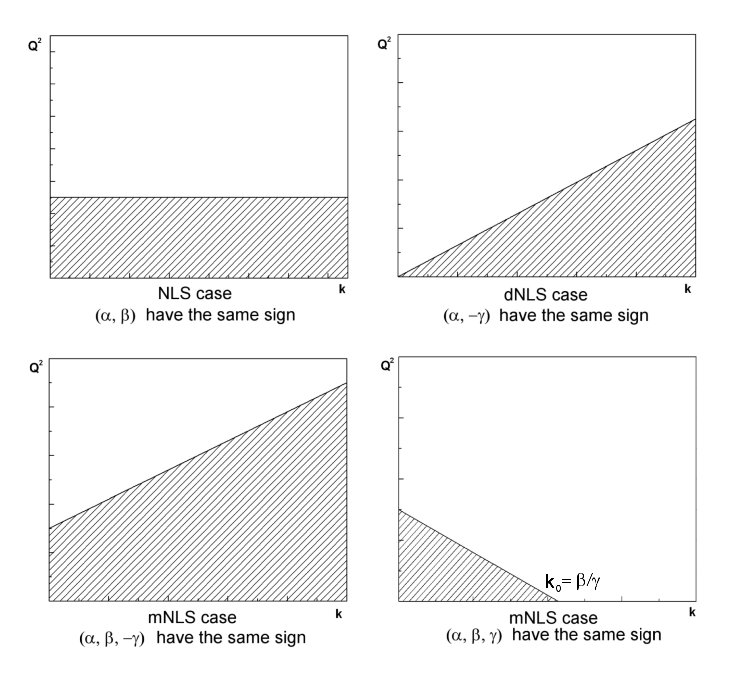
\includegraphics[width=0.8\textwidth]{xNLS_DAMI}
\caption{This is a sample picture taken from RJP volume \textbf{50}(1-2) from page 129 (2005).It illustrates (hashed areas) the instability domains for a series of nonlinear Schr\"odinger equations determined using the deterministic approach to modulational instability.}
\label{pic1}
\end{figure}

Another environment with special formatting in our style is the \textit{table} environment, a sample of which is table \ref{table1}. Please, do notice that the caption of tables is usually placed before the main body and therefore, you are required to write the \texcom{caption\{...\}} command immediately after \texcom{begin\{table\}...} !
\begin{table}[h!t]%
\caption{This table is taken from RJP volume \textbf{50}(1-2) from page 43 (2005). It gives the ``
\textit{number of bound states dependence on the radius of space curvature for $\alpha = 0.005$, $U_0 = 1$}''.}
\centering
\begin{tabular}{|c|c|}
\hline
Value $\rho$ & Value $\varepsilon$ \cr
\hline
$\rho = 50$ & -- \cr
$\rho = 100$ & -- \cr
$\rho = 250$ & $\varepsilon_1 = 0.0289$ \cr
$\rho = 400$ & $\varepsilon_1 = 0.3772$ \cr
$\rho = 1000$ & $\varepsilon_1 = 0.4142$, $\varepsilon_2 = 0.8495$ \cr
\hline
\end{tabular}
\label{table1}
\end{table}

As RJP is a physics journal, an important part of the scientific language used in the publication is constituted by equations. One of the main reason for which the developer decided to include the AMS style within the RJP style is the appropriate formatting of the mathematical environments. For instance the \textit{split} or \textit {align} environment is recommended as a very good replacement of the \textit{eqnarray} environment. You can see the difference between \textit{split} and \textit{eqnarray} in equation \eqref{eq1} and \eqref{eq2}, respectively. An even better layout may be obtained if one uses the 
\textit{aligned} environment inside the \textit{equation} or the \textit{multline} environment as in \eqref{eq2b}, respectively \eqref{eq2c}.
\begin{equation}\label{eq1}\begin{split}
S_{0}&[A^{\mu },\dot{A}^\mu,\phi ]=\int d^{4}x\mathcal{L}=\int
d^{4}x\ (-\frac{1}{4}F_{\mu \nu }F^{\mu \nu }- \\
&-k~\partial _{\lambda }F^{\alpha \lambda }\partial _{\rho }F_{\alpha }^{\rho
}+\frac{1}{2}(\partial _{\mu }\phi -mA_{\mu })(\partial ^{\mu }\phi -mA^{\mu
}))
\end{split}\end{equation}
\begin{eqnarray}
& &S_{0}[A^{\mu },\dot{A}^\mu,\phi ]=\int d^{4}x\mathcal{L}=\int
d^{4}x\ (-\frac{1}{4}F_{\mu \nu }F^{\mu \nu }- \label{eq2} \\
& &-k~\partial _{\lambda }F^{\alpha \lambda }\partial _{\rho }F_{\alpha }^{\rho
}+\frac{1}{2}(\partial _{\mu }\phi -mA_{\mu })(\partial ^{\mu }\phi -mA^{\mu
})) \nonumber
\end{eqnarray}
\begin{equation}\label{eq2b}\begin{aligned}
S_{0}&[A^{\mu },\dot{A}^\mu,\phi ]=\int d^{4}x\mathcal{L}=\int
d^{4}x\ (-\frac{1}{4}F_{\mu \nu }F^{\mu \nu }- \\
&-k~\partial _{\lambda }F^{\alpha \lambda }\partial _{\rho }F_{\alpha }^{\rho
}+\frac{1}{2}(\partial _{\mu }\phi -mA_{\mu })(\partial ^{\mu }\phi -mA^{\mu
}))
\end{aligned}\end{equation}
\begin{multline}\label{eq2c}
S_{0}[A^{\mu },\dot{A}^\mu,\phi ]=\int d^{4}x\mathcal{L}=\int
d^{4}x\ (-\frac{1}{4}F_{\mu \nu }F^{\mu \nu }- \\
-k \partial _{\lambda }F^{\alpha \lambda }\partial _{\rho }F_{\alpha }^{\rho
}+\frac{1}{2}(\partial _{\mu }\phi -mA_{\mu })(\partial ^{\mu }\phi -mA^{\mu
}))
\end{multline}
Please, be advised that since 2012 the RJP document class issues errors whenever more than 3 \textit{eqnarray} environments are encountered in one section of an article! This measure was required due to abusive use of this environment which hinders the processing of documents before publishing.

The AMS style also allows one to easily make use of subequations
\begin{subequations}
\label{ein}
\begin{align}
\frac{\ddot a_2}{a_2} +\frac{\ddot a_3}{a_3} +\frac{\dot
a_2}{a_2}\frac{\dot
a_3}{a_3} - \frac{n^2}{a_3^2} &= \kappa T_{1}^{1}\,, \label{11}\\
\frac{\ddot a_3}{a_3} +\frac{\ddot a_1}{a_1} +\frac{\dot
a_3}{a_3}\frac{\dot
a_1}{a_1} - \frac{m^2}{a_3^2} &= \kappa T_{2}^{2}\,, \label{22} \\
\frac{\ddot a_1}{a_1} +\frac{\ddot a_2}{a_2} +\frac{\dot
a_1}{a_1}\frac{\dot
a_2}{a_2} + \frac{m n}{a_3^2} &= \kappa T_{3}^{3}\,, \label{33} \\
\frac{\dot a_1}{a_1}\frac{\dot a_2}{a_2} +\frac{\dot a_2}{a_2}
\frac{\dot a_3}{a_3} + \frac{\dot a_3}{a_3}\frac{\dot a_1}{a_1} -
\frac{m^2 - m n + n^2}{a_3^2} &=
\kappa T_{0}^{0}\,, \label{00}\\
m \frac{\dot a_1}{a_1} - n \frac{\dot a_2}{a_2} - (m - n) \frac{\dot
a_3}{a_3} &= \kappa T_{3}^{0}\,. \label{03}
\end{align}
\end{subequations}
though one should consult the AMS user guide \cite{amsug} when special features like splitting subequations between subsequent pages are needed (see \cite{amsug} ver. 2.0, revised 2002, p. 9-10). Please notice that the \textit{subequations} environment presents the advantage of referencing both the whole group of equations \eqref{ein} or each of the sub-equations individually, \textit{e.g.} \eqref{33}. Of course, there are other mathematical AMS environments that the author may use in their papers and to learn about them one should consult the afore-mentioned user guide.

\section{Instead of Conclusions}

The current style provides a few elements of both authenticity for us (the headers and footers) as well as a way for you, the author, to certify (to third parties) the submission of a manuscript to our journal. Most of the formatting is done automatically in the background so you \textbf{must not} interfere with elements such as page layout parameters, spacing parameters used in various environments or font sizes. In 2012 a minimal mechanism was implemented to detect page layout modification. Upon detection the document output is stopped until the author removes the preamble commands or the packages causing the page geometry modification. We admit however that in certain conditions (especially when lots of floating environments (figures and tables) are used) the author may need to issue special commands to force the output of floats on specific pages (such commands are \textbackslash clearpage, \textbackslash newpage, etc.). Of course these commands are allowed in your \LaTeX ~code. However, please do not 
drastically modify font sizes used in various environments nor force vertical or horizontal space in your article! Such actions will be considered an abuse and will hinder our efforts to publish your accepted paper as soon as possible, most likely leading to indefinite delays in publication. We also recommend that you do a spelling before submitting your article and use the \textbackslash hyphenation command (or hyphenation marks) whenever necessary.

These recommendations should be taken into account together with the instructions for authors available for consulting on the Romanian Journal of Physics web site when submitting articles written in \LaTeX ~to our journal. Please, be advised that failure to comply may lead to indefinite delays in the publication of your submitted article even if the referees gave you a positive recommendation!

The current style (Dec. 2013) is being constantly improved and patched, therefore comments and contributions to the development of the code as well as help in debugging specific issues is and will always be highly regarded by our editorial team!

Last but not least, we give some \textbf{real} references to works by scientists who became very well-known (publicly) during the year 2010 in physics \cite{nobelphys1, nobelphys2, nobelphys3} and mathematics \cite{fields1,fields2,fields3}.

\section{Log of changes}

\subsection{\NoCaseChange{\texttt{version 2.0 r2018a}}}
\begin{itemize}
\item[-] disable use of bibliographic data bases in \texttt{.bib} format on EB decision
\end{itemize}

\subsection{\NoCaseChange{\texttt{version 2.0 r2017b}}}
\begin{itemize}
\item[-] changed bibliography code to avoid breaking bibliographic entries between pages
\end{itemize}

\subsection{\NoCaseChange{\texttt{version 1.1 r2016a}}}
\begin{itemize}
  \item[-] added \texttt{mathlines} option to \texttt{lineno} package in order to count also lines with mathematical formula
  \item[-] bilbliography style \texttt{rjpstyle(.bst)} was customized to improve parsing of bibtex bibliography data bases. It is recommended that empty fields in records from such data bases should be written as \texttt{$<$field name$>$ = \{\},}
\end{itemize}

\subsection{\NoCaseChange{\texttt{version 1.1 r2015a}}}
\begin{itemize}
  \item[-] added \texcom{rjpNoMark} command (see text above for details)
  \item[-] change citation management package from \texttt{cite} to \texttt{natbib}
  \item[-] included \texttt{hyperref} package to enable internal and external links in produced PDF files
  \item[-] two new commands \texcom{arxiv} and \texcom{doi} are introduced in order to facilitate linking the references to external resources.\\
  \texcom{arxiv} has two arguments, one of which is mandatory and must be the article number in the \earXiv~ system. The optional argument is the 
  domain abbreviation. \\
  \texcom{doi} takes also two arguments, the mandatory one being the Digital Object Identifier (DOI) of the referenced external resource while the optional argument can be whatever text the user wants to be displayed for the link in the PDF document. When not provided a default text is inserted of the form \texttt{DOI:$<$doi-number$>$}.
\end{itemize}

\subsection{\NoCaseChange{\texttt{version 1.0 r2013b}, class date: November, 2013}}
\begin{itemize}
 \item[-] adjusted alignment of subsequent lines in a bibliography entry
 \item[-] adjourned this document and clean-up of \textit{rjp\_mathdefs.tex} auxiliary macro file.
\end{itemize}

\subsection{\NoCaseChange{\texttt{version 1.0 r2013a}, class date: February 9, 2013}}
\begin{itemize}
 \item[-] command \texttt{\textbackslash email} is available in \texttt{\textbackslash affil} command
\end{itemize}

\subsection{Release \NoCaseChange{2012c}}
\begin{itemize}
\item[-] replaced \textbf{color} package by the modern, improved \textbf{xcolor} package
\item[-] the class now uses by default the \textbf{lineno} package in order to facilitate the reviewing process by marking the lines in the manuscripts
\item[-] the \textbf{graphicx} package is now instructed to search for figures in \textit{figs} directory under the current path, \textit{i.e.} \texttt{\small ./figs/}
\end{itemize}

\section{Macros available in \NoCaseChange{\textit{rjp\_mathdefs.tex}}}

The list below contains the \LaTeX\ macros available through the \textit{rjp\_mathdefs.tex} file. Please, do consider these macros and try to avoid redefining or clashing with their names in your own contribution. Contrarily to limitations on the definition and use of user macros which other journals enforce, most of the macros described below are introduced using the \texcom{providecommand} command which gives you the liberty to overwrite them at will. However, we would very much appreciate and acknowledge if you minimize in your contribution the use of packages or user macros the functionality of which is not needed to generate the final PDF document (\ie\ before sending your contribution please, take a few extra minutes to remove un-used \texcom{usepackage\{...\}} and macros from your \LaTeX\ file).

\noindent\texttt{\textbackslash beq ... \textbackslash eeq} -- these shortcut command replace the start and end commands for the \texttt{equation} environment; \texttt{beq} has an optional argument which is used as the label of the equation, therefore avoid starting your equation with the '[' character place right after \texcom{beq}. \\
\noindent\texttt{\textbackslash beqn ... \textbackslash eeqn} -- shortcut command for the star version of the equation environment  \\
\noindent\texcom{jsn},...\texcom{jds},...\texcom{jcd} -- the complete list of Jacobi elliptic functions defined by pre-pending \texttt{j} to their names as consecrated in literature \\
\noindent\texcom{ddiv} and \texcom{grad} -- if you prefer to avoid denoting the operators using $\nabla$.  \\
\noindent\texcom{ee} -- the transitional number $\mathrm{e} = 2.7178...$ as a mathematical operator (straight font) \\
\noindent\texcom{Tr} -- the matrix trace operator in straight font \\
\noindent\texcom{Img}/\texcom{Rel} -- to specify the imaginary part coefficient/real part for a complex quantity $z$ so that  $z = \mathrm{Re} z + i\; \mathrm{Im} z$ \\
\noindent\texcom{sgn} -- the sign function in straight font \\
\noindent\texcom{cosec} -- the co-secant trigonometric function ($1/\cos$) \\
\noindent\texcom{artanh} -- the inverse of the $\tanh$ hyperbolic function ($\tanh^{-1}$) \\
\noindent\texcom{sech} and \texcom{cosech} -- hyperbolic functions $1/\cosh$ and $1/\sinh = \mathrm{csch}$, respectively. \\
\noindent\texcom{eps} -- for $\varepsilon$ \\
\noindent\texcom{cc} -- to input complex conjugate abbreviation in math and text mode followed by a small (non-breakable) blank \\
\noindent\texcom{ict} -- to input $\mathcal{C}$ in math mode and \texttt{C} in text mode as a symbol for an arbitrary integration constant \\
\noindent\texcom{pd} -- shortcut for $\partial$, partial derivative in math mode \\
\noindent\texcom{fd} -- output the full derivative symbol (d) in straight font in math mode (very useful for writing nice derivatives and integrals) \\
\noindent\texcom{bra}, \texcom{ket} and \texcom{braket} -- to print out bra and ket wave-vectors with correct scaling of the surrounding symbols (1 argument) or the quantum matrix element of an operator given as first argument between two states given as argument 2 and 3 for bra and ket states respectively \\
\noindent\texcom{fudbud[5]}, \texcom{fubu[3]}, \texcom{fdbu[3]},
\texcom{fdbd[3]}, \texcom{fubd[3]} -- series of commands to arrange more conveniently upper and lower indexes in front and after a central symbol/token given first argument of the commands; the names are derived from ``front up-down, back up-down'' and the corresponding letter combination dictates also the order of the remaining arguments, \textit{e.g.} \texcom{fubu\{A\}\{i\}\{j\}} will produce ${\!\;}^{i}\!\!A^{j}$.\\
\textit{Set of commands for abbreviation formatting}:\\
\texcom{eg} $\to$ \textit{e.g.}; \texcom{ie} $\to$ \textit{i.e.}; \texcom{etal} $\to$ \textit{et al.}

This list of macros is meant to grow and evolve with the requirements of the Romanian Journal of Physics publishing authors so please, do not hesitate to contact the developer of this style for bugs or special commands that you want us to consider for inclusion. Also, please, take into account that the list published here may not always be up to date.

%\subsection{Release \NoCaseChange{}}

%\begin{itemize}
%\item[-]
%\end{itemize}

\begin{acknowledgement}
The author(s) would like to dedicate this class to the memory of \linebreak
\framebox{Acad. Dr. Horia Scutaru} a great scientist and supporter of innovation at RJP. A.T.G. would like to acknowledge the help received from Mrs. Margareta Oancea and the members of the technical department at the Romanian Academy Publishing House, in principal, in specifying a \LaTeX\ format that matches as close as possible the MS Word template that RJP uses officially, but also for carefully and patiently correcting the various versions produced during development. Last but not least, the authors owe gratitude to those who made possible that Donald Knuth's \cite{dknuthhp} complex but rigorous \TeX \cite{knuth,teximpacient} evolve into the friendlier \LaTeXe (of course names like Leslie Lamport \cite{leslie} or the people in the \LaTeX3 project led by Frank Mittelbach \cite{mittelbach,ltexclass,ltexshort,ltexclass2} come to mind). A big ``Thanks!'' goes to all the web sites, forums and message lists maintainers out there on the internet for the 
documentation and examples they shared with the world in the obvious effort of teaching people about the ways and wonders of beautiful typesetting (a small part of these resources are in Refs. \cite{texrefex,eijkhout,texcookbook,pagelayout,tug,stacko,web1,web2,web3,web4,web5,web6,web7,web8}).
\end{acknowledgement}

\begin{thebibliography}{99}
\bibitem{knuth}D. E. Knuth, D. R. Bibby, ``\textit{The \TeX book}'', 20th edn. (AMS \& Addison-Wesley Publ. Co., 1991).

\bibitem{dknuthhp} D. E. Knuth homepage: \href{http://www-cs-faculty.stanford.edu/~knuth/}{\small\ttfamily www-cs-faculty.stanford.edu/\~{}knuth}.

\bibitem{eijkhout} V. Eijkhout, ``\textit{\TeX~ by Topic, A \TeX nician's Reference}'' (electronic ver. 1.0, 2001).

\bibitem{texcookbook} ``\textit{\TeX Cookbook}'' (MathPro Press, 1989; \href{http://www.mathpro.com/math/MathPro.html}{\small\ttfamily www.mathpro.com/math/MathPro.html}).

\bibitem{texrefex} D. Bausum, ``\textit{\TeX: Reference and Examples}'' 
(\href{http://www.tug.org/utilities/plain/cseq.html}{\small\ttfamily www.tug.org/utilities/plain/cseq.html}).

\bibitem{teximpacient} P. W. Abrahams, K. A. Hargreaves, K. Berry, ``\textit{\TeX~ for the Impatient}'' (Addison-Wesley Publ. Co., 2003).

\bibitem{tug}\TeX  \textit{Users Group}: \href{http://www.tug.org/tutorials/}{\small\ttfamily www.tug.org/tutorials/}.

\bibitem{leslie} L. Lamport, ``\textit{\LaTeX. A Document Preparation System}'', 2nd edn. (Addison-Wesley Publ. Co., 1994).

\bibitem{mittelbach} F. Mittelbach, M. Goossens (J. Braams, D. Carlisle, C. Rowley), ``\textit{The \LaTeX~ Companion}'', 2nd edn. (Addison-Wesley, Boston, 2004).

\bibitem{ltexclass} The \LaTeX3 Project, ``\textit{\LaTeXe~ for Class and Package Writers}'' (1999).

\bibitem{ltexshort} T. Oetiker, H. Partl, I. Hyna, E. Schlegl, ``\textit{The Not So Short Introduction to \LaTeXe}'' (ver. 4.31, June 24, 2010).

\bibitem{ltexclass2} The \LaTeX3 Project, ``\textit{\LaTeXe~ for Authors}'' (2001).

\bibitem{pagelayout} P. van Oostrum, ``\textit{Page Layout in \LaTeX}'' (\href{http://www.cs.ruu.nl/people/piet}{\small\ttfamily www.cs.ruu.nl/people/piet}).

\bibitem{web1}A. J. Hildebrand, \href{http://www.math.uiuc.edu/~hildebr/tex/}{\small\ttfamily www.math.uiuc.edu/\~{}hildebr/tex}.

\bibitem{web2} \href{http://zoonek.free.fr/LaTeX/}{\small\ttfamily zoonek.free.fr/LaTeX}.

\bibitem{web3} \href{http://amath.colorado.edu/documentation/LaTeX}{\small\ttfamily amath.colorado.edu/documentation/LaTeX}.

\bibitem{web4} \href{http://www-h.eng.cam.ac.uk/help/tpl/textprocessing/}{\small\ttfamily www-h.eng.cam.ac.uk/help/tpl/textprocessing}.

\bibitem{web5} \href{http://latex.computersci.org/}{\small\ttfamily latex.computersci.org}.

\bibitem{web6} S. Kottwitz, \href{http://texblog.net/}{\small\ttfamily texblog.net}.

\bibitem{web7} \href{http://www.personal.ceu.hu/tex/}{\small\ttfamily www.personal.ceu.hu/tex/}.

\bibitem{web8} The UK \TeX~ Archive: \href{http://www.tex.ac.uk/}{\small\ttfamily www.tex.ac.uk}.

\bibitem{stacko} Stack Overflow: \href{http://stackoverflow.com/tags}{\small\ttfamily stackoverflow.com/tags}.

\bibitem{amsug} User's Guide for the \textit{amsmath} Package: \href{ftp://ftp.ams.org/pub/tex/doc/amsmath/amsldoc.pdf}{\small\ttfamily ftp.ams.org/pub/tex/doc/amsmath/amsldoc.pdf}.

\bibitem{nobelphys1}F. Guinea, M. I. Katsnelson, A. K. Geim, Nature Physics \textbf{6}, 30--33 (2010).

\bibitem{nobelphys2}A. K. Geim, Science \textbf{324}, 1530--1534 (2009).

\bibitem{nobelphys3}D. C. Elias, R. R. Nair, T. M. G. Mohiuddin, S. V. Morozov, P. Blake, M. P. Halsall, A. C. Ferrari, D. W. Boukhvalov, M. I. Katsnelson, A. K. Geim, K. S. Novoselov, Science \textbf{323}, 610--613 (2009).

\bibitem{fields1}G. Toscani, C. Villani, Comm. Math. Phys. \textbf{203}(3), 667--706 (1999).

\bibitem{fields2}I.M. Gamba, V. Panferov, C. Villani, Comm. Math. Phys. \textbf{246}(3), 503--541 (2004).

\bibitem{fields3}C. Villani, Rev. Matem. Iberoam. \textbf{15}(2), 335--352 (1999).

\end{thebibliography}


\end{document}